\documentclass{vldb}

\usepackage{amsmath,amssymb}
\usepackage{stmaryrd}
\usepackage{graphicx}
\usepackage{color}
\usepackage{hyperref}

\newcommand{\comment}[1]{}
\newcommand{\tinysection}[1]{\noindent{\bf #1.}}
\newcommand{\tuple}[1]{{\langle#1\rangle}}
\newcommand{\todo}[1]{\textcolor{red}{#1}}
\newcommand{\note}[1]{\textcolor{blue}{#1}}

\newcommand{\compiler}{DBToaster}
\newcommand{\spe}{Jasper}
\newcommand{\driver}{JDBC}

\newcommand{\targetlang}{Java}
\newcommand{\dsl}{QueryDSL}
\newcommand{\dslurl}{\url{http://www.querydsl.com}}

%\newcommand{\targetlang}{Scala}
%\newcommand{\dsl}{ScalaQuery}
%\newcommand{\dslurl}{\url{http://http://scalaquery.org}}

\begin{document}
\title{Algorithmic Trading on Order Books with Embedded Queries and Synthesized
Stream Engines}
\numberofauthors{3}
\author{
\alignauthor
Oliver Kennedy\\
\affaddr{EPFL, Cornell}\\
\email{oliver.kennedy@epfl.ch}
\alignauthor
Yanif Ahmad\\
\affaddr{Johns Hopkins University}\\
\email{yanif@jhu.edu}
\alignauthor
Christoph Koch\\
\affaddr{EPFL}\\
\email{christoph.koch@epfl.ch}}
\maketitle

\begin{abstract}
Moo.
\end{abstract}

\section{Introduction}



In recent years, algorithmic trading systems have come to account for a majority
of volume traded at the major US and European financial markets (for instance,
for 73\% of all US equity trading volume in the first quarter of 2009
\cite{Iati2009}). The success of automated trading systems depends critically on
strategy processing speeds: trading systems that react faster to market events
tend to make money at the cost of slower systems. Unsurprisingly, algorithmic
trading has become a substantial source of business for the IT industry; for
instance, it is the leading vertical among the customer bases for high-speed
switch manufacturers (e.g., Arista \cite{Becht2010}) and data stream processing.




A typical algorithmic trading system is run by mathematicians who develop
trading strategies and by programmers and systems experts who implement these
strategies to perform fast enough, using mainly low-level programming languages
such as C. Developing trading strategies requires a feedback loop of simulation,
back-testing with historical data, and strategy refinement based on the insights
gained. This loop, and the considerable amount of low-level programming that it
causes, is the root of a very costly {\em productivity bottleneck}\/: in fact,
the number of programmers often exceeds the number of strategy designers by
an order of magnitude.


Trading algorithms often perform a considerable amount of data crunching
and statistical processing that could in principle be implemented using SQL
views, coupled with some relatively straightforward control and trading logic.
%
Differently from other areas of finance such as technical analysis,
where stream processing engines
\cite{abadi-vldbj:03,motwani-cidr:03} can be applied,
data processing in trading algorithms using views cannot be performed by DBMS or
data stream processing systems today: the former are not able to (1) {\em update
their views at the required rates}\/ (for popular stocks, hundreds of orders per
second may be executed, even outside burst times) and the latter are not able to
(2) {\em maintain large enough data state}\/ and support suitable query
languages (non-windowed SQL aggregates) on this state.

%
A data management system that could handle these two requirements would yield a
very substantial productivity increase that can be directly monetized -- the
holy grail of algorithmic trading.

Trading algorithms often perform a considerable amount of data crunching that
could in principle be implemented as SQL views, but cannot be achieved by DBMS
or data stream processing systems today: DBMS are not able to (1) {\em update
their views at the required rates}\/ (for popular stocks, hundreds of orders per
second may be executed, even outside burst times) and stream engines are not
able to (2) {\em maintain large enough data state}\/ and support suitable query
languages (non-windowed SQL aggregates) on this state.
A data management system fulfilling these two requirements would yield a very
substantial productivity increase that can be directly monetized -- the holy
grail of algorithmic trading.



To understand the need to maintain and query a large data state, note that
many stock exchanges provide a detailed view of the market microstructure
through complete bid and ask {\em limit order books}. The bid order book is a
table of purchase offers with their prices and volumes, and correspondingly the
ask order book indicates investors' selling orders. Exchanges execute trades by
matching bids and asks by price and favoring earlier timestamps. Investors
continually add, modify or withdraw limit orders, thus one may view order books
as relational tables subject to high update volumes. The availability of order
book data has provided substantial opportunities for automatic algorithmic
trading.





To illustrate this, we describe the Static Order Book Imbalance (SOBI) trading
strategy. SOBI computes a volume-weighted average price (VWAP) over those orders
whose volume makes up a fixed upper $k$-fraction of the total stock volume in
both bid and ask order books. SOBI then compares the two VWAPs and, based on
this, predicts a future price drift (for example a bid VWAP larger than an ask
VWAP indicates demand exceeds supply, and prices may rise). For simplicity, we
present the VWAP for the bids only:



\begin{verbatim}
select avg(b2.price * b2.volume) as bid_vwap
from   bids b2
where  k * (select sum(volume) from bids)
         > (select sum(volume) from bids b1
            where b1.price > b2.price);
\end{verbatim}
\comment{
Focusing on the $k$-fraction of the order book closest to the current price
makes the SOBI strategy less prone to attacks known as {\em axes}\/ (large
tactical orders far from the current price that will thus not be executed but
may confuse competing algorithms).
}


Coming back to our two desiderata, for trading algorithms to be successful, (1)
views such as VWAP need to be maintained and monitored by the algorithms at or
close to the trading rate. However, (2) the views cannot be expressed through
time-, row- or punctuation-based window semantics.






\clearpage

\section{The DBToaster Platform}

The \compiler\ project investigates processing techniques and architectural
design for dynamic data management systems. Its two core research themes are
that of incremental query processing, and program synthesis where we can tailor
the design of system internals to yield lightweight, efficient data management
tools. Algorithmic trading, where specialized engines abound, is a natural use
case for \compiler. High-frequency data ingestion and the competitive advantage
of low latencies has led to widespread use of low-level code and
processing hardware such as FPGAs. We describe the computational and software
development aspects of the \compiler\ platform and toolchain below.

\tinysection{Dynamic Data Management}
\compiler\ constructs dynamic data management tools that process database
updates as incrementally as possible. Its query model is identical to that of
view maintenance \todo{[IVM citations]}, where given a SQL query on a database,
it generates a program to maintain query results as the database changes. Its
novelty lies in the nature of this maintenance program, and its use of
\textit{agile} views and \textit{multi-level} view maintenance.
\todo{Blurb about agile views, etc.}

\tinysection{Query Engine Compilation and Synthesis}
The \compiler\ compilation framework uses two internal representations to
synthesize stream engines, the first is a query calculus used to compute
higher-level delta queries as mentioned above and for a variety of
simplifications relating to constant folding, unification, variable elimination
and factorization. The second representation is a collection-oriented functional
language, extended with constructs such as persistence and resource annotations
to better utilise the hardware for computations performed by queries.

\todo{SQL queries, preaggregation, construction of incremental plan 
(polynomialization, delta transformation, simplification, repeat), low-level
compilation}

\todo{Diagram of platform: query, compiler, code generator backends, use of
generated code in runtimes}

In its current incarnation, \compiler\ acts as a one-shot compiler that
transforms standard SQL queries into incremental programs as described above.
\compiler\ supports an extensible, retargettable code generator that currently
has support for running incremental programs in a variety of imperative or
functional languages (C++, Java, OCaml), as well as on massively parallel
processing infrastructures (Hadoop, and DBToaster Cumulus, a fine-grained
shared-nothing streaming runtime currently under development). In this
demonstration, we will compile SQL queries to Java, for use in our
coarse-grained stream engine, Jasper (we describe this in more detail below).


\tinysection{Programming with DBToaster} 
The benefits of type-safety and the ability to analyse and optimize expressions
offered by language integrated queries and embedded domain specific query
languages has greatly improved the development process for applications
interacting with data management systems. To this day however, the focus has
been on using databases either as a persistence layer \todo{[xxx]}, or as
coprocessors \todo{[Ferry]}. The \compiler\ project faces outwards from data
management techniques, viewing such trends as an opportunity to export
and embed query processing, optimization, indexing and storage,
transaction management, and concurrency directly into application code.

\note{Comment on the advantages of native code querying, esp. in terms of UDFs
(aka abstraction in the PL literature).}


Our current focus is on main-memory view maintenance. \compiler\ uses an
embedded SQL DSL called \dsl\ (\dslurl) to integrate with application code
written in \targetlang.
\todo{Simple \dsl\ example with \targetlang\ app logic.}
\dsl\ generates SQL query strings in a type-safe manner and executes them
over a \driver\ connection. We are developing a bare-bones \driver\ driver to
support the execution of SQL queries, which involves (just-in-time) query
compilation via the \compiler\ compiler into \targetlang\ code, dynamic loading
of the \targetlang\ classes corresponding to the newly created query engine, and
finally engine execution.


Applications can access
result sets which are internally backed by the data structures maintained by
\compiler\ engines. In addition to the standard pull-based interfaces provided
by the JDBC API, we provide an API for push-based notifications and application
code execution via callbacks. Other event-driven mechanisms that we will develop
in the future include proxy datastructures and futures \todo{[CIDR]}. To
summarize, in this demonstration, we will show how \compiler\ can be used to
create a pure Java application that embeds an in-process relational stream
engine.


\tinysection{The DBToaster Runtime}
In addition to supporting direct application use of queries, \compiler\ provides
a query runtime to facilitate managed execution of queries, in particular to
provide a coarse-grained approach to scaling query workloads by performing
resource allocation and distributed execution. The \compiler\ runtime is a
distributed stream processing engine called \spe\ which has been inspired by
earlier efforts on the Borealis project~\todo{[CIDR 05]}. \spe\ is
implemented in Java making it well suited to JVM-based target
languages for \compiler, and internally invokes \compiler\ to generate
operators. Our operators are arbitrarily complex queries that may
perform nesting, multiway joins, essentially the full fragment of SQL
supported by \compiler, enabling the specification of operators or
\textit{modules} in a declarative language. \spe\ can provide window query
functionality around modules (which simply invoke insert or delete triggers in
\compiler\ code), as well core runtime and distribution mechanisms such as
checkpointing, or migrating operators (given that all \compiler\ code includes
automatic serialization of internal state).

\todo{What kind of coupling do we provide for application and queries with this
managed runtime? Are apps also compiled into migratable modules, or do we
provide a layer of indirection at their interaction to let us do whatever we
want under the hood?}

\todo{Architecture diagram and components: data structures, compiling
operators, Jasper (a simple, generic stream processor), external windowing of
queries with Jasper+DBToaster}


\section{Algorithmic Trading}
In this demonstration, we will use an end-to-end algorithmic trading platform to
demonstrate the advantages of coupling application and data management logic, in
addition to scaling out data processing. For example, we can use application
logic to coordinate messaging and execute protocols, functionality that
traditionally does not concern data management systems, while still taking
advantage of efficient processing techniques once we have structured data in
hand. Our algorithmic trading platform will provide tools to simulate markets,
with the primary form of data being order books capturing buy and sell orders
from market participants. The platform consists of three high-level components:
i) a stock exchange simulator, ii) a trading platform runtime built on top of
the \compiler\ runtime that executes trading algorithms (algos), and iii) a
trading workstation where users can interactively enter, modify and visualize
the behavior of their algos. We describe these components before discussing the
workflow.

\tinysection{Stock exchange simulator} In order to validate the efficacy of
their algos, many trading firms perform simulations, or backtesting of their
algos in a controlled setting. Our trading platform will include a stock
exchange simulator whose role is to match buyers to sellers that place limit
and market orders. Matching occurs on order books, which are two relations
maintained internally within electronic exchanges such as NASDAQ and NYSE, and
include attributes such as an order identifier, security symbol, price and
volume, as seen when adding orders in the NASDAQ Totalview-ITCH format
\todo{[NASDAQ]}.

While the core matching logic performed by an exchange is well defined, the
underlying challenge is to provide an environment for testing algos that
reflects actual markets as best possible. Trading firms frequently use
historical traces of actual events on markets as test cases, thus our simulator
supports replay functionality, and critically, combines these historical traces
with actions placed by the algos undergoing testing. The use of historical
traces also enables simulation at scale, as opposed to running algos to simulate
the combined behavior of each individual broker trading on the market.

\todo{Implementation with which tools?}

\tinysection{Trading algorithms}
The goal of our trading platform is to facilitate simplified and rapid
development of trading algorithms. In many trading firms, after teams of
researchers develop prototypes of algorithms, software engineers painstakingly
transform such algorithms into efficient low-level code for deployment on
trading platforms. Our view is that a software stack coupling declarative query
capabilities integrated with general purpose programming will greatly improve
this development cycle. In this demonstration, we will provide examples of algos
implemented using queries to perform basic analytical computations, encompassed
by order routing logic to submit and be notified of orders occurring at the
stock exchange. \todo{Tie in with description of how apps and queries interact
on the runtime.}

In particular, we will provide a set of predefined indicators on
order books, such as momentum, volatilities, volume-weighted average prices
(VWAP), order book imbalances (SOBI, NOII), market aggregate order
aggressiveness (MAOA), expressed as and composed with SQL queries.

\todo{Examples of parts of algos that are difficult to express in SQL?}

\tinysection{Trading workstation}

\tinysection{Algorithmic trading workflow}

\todo{Architecture diagram}

\begin{figure}
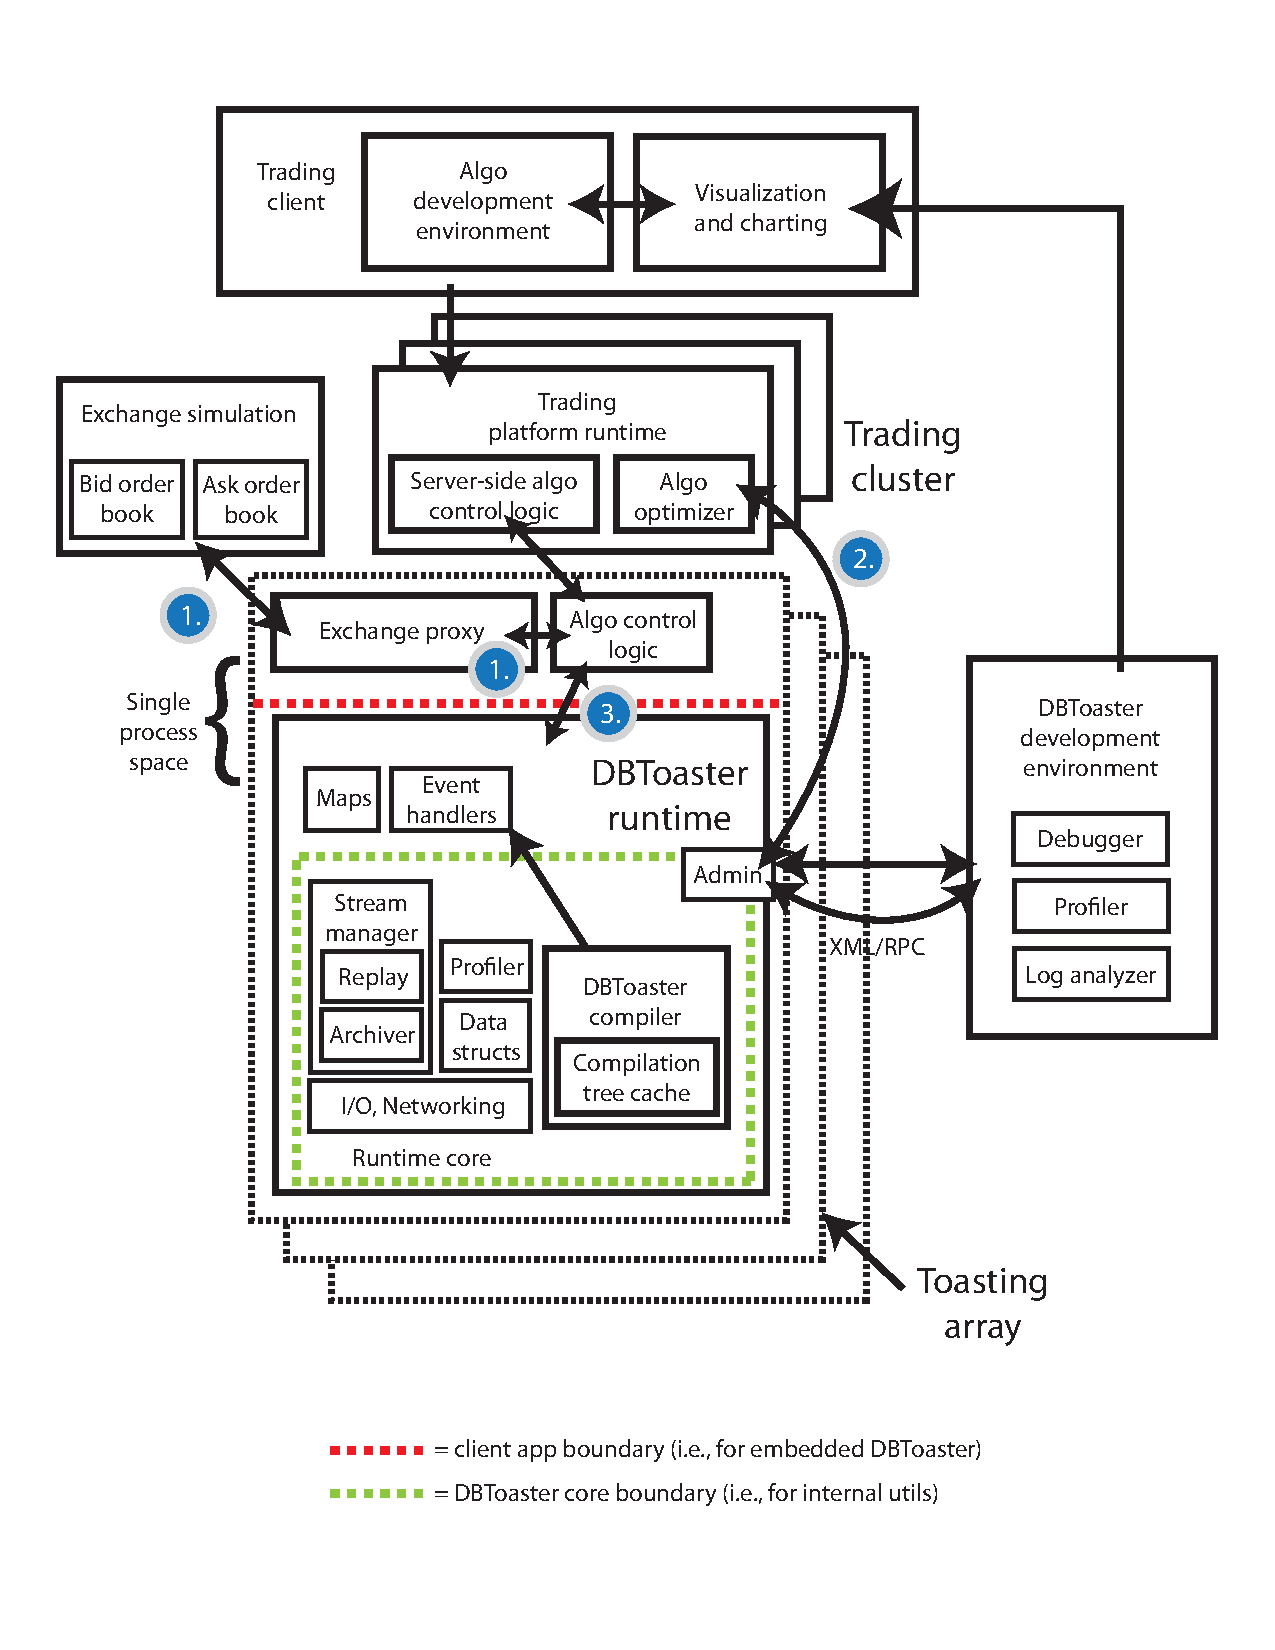
\includegraphics[scale=0.38]{figures/finapp}
\end{figure}


\begin{itemize}
  \item Example algorithms: VWAP, Ax finder, market making, icebergs, sniping.
  \item Advanced algorithms: combining level I and level II algorithms,
  combining alternate data sources, e.g. news feeds, twitter feeds. Would be
  nice to have learning algorithms and maintenance for them.
  \item Portfolio management.
  \item Exchange simulation: using histories to create alternate realities
  \item Algorithm simulation and backtesting: creating multiple agents that
  interact with each other
  \item Trading workstation: \todo{declarative visualization would be awesome..}
\end{itemize}

\section{Demo Scenario}

\todo{Demo screenshots}

\tinysection{Audience Participation}

\end{document}
